\chapter{The Scenarios Manager}
\label{chap:scenarios-manager}

\section{Running a Simulation}

Once a project has been developed, including the data to be used in it, and
the model system has been configured and the parameters for the models
estimated, the next step is to create and run a scenario.  In the
eugene\_gridcell project, a baseline scenario has already been created and
is ready to run.  To run this scenario, in the Scenario Manager,
right-click with the mouse on the Eugene\_baseline entry and select
``Run this Scenario.''  At this point, a frame should appear in the
right hand side of the Opus window, as shown in Figure
\ref{fig:scenario-manager-start-run}.

\begin{figure}[htp]
\begin{center}
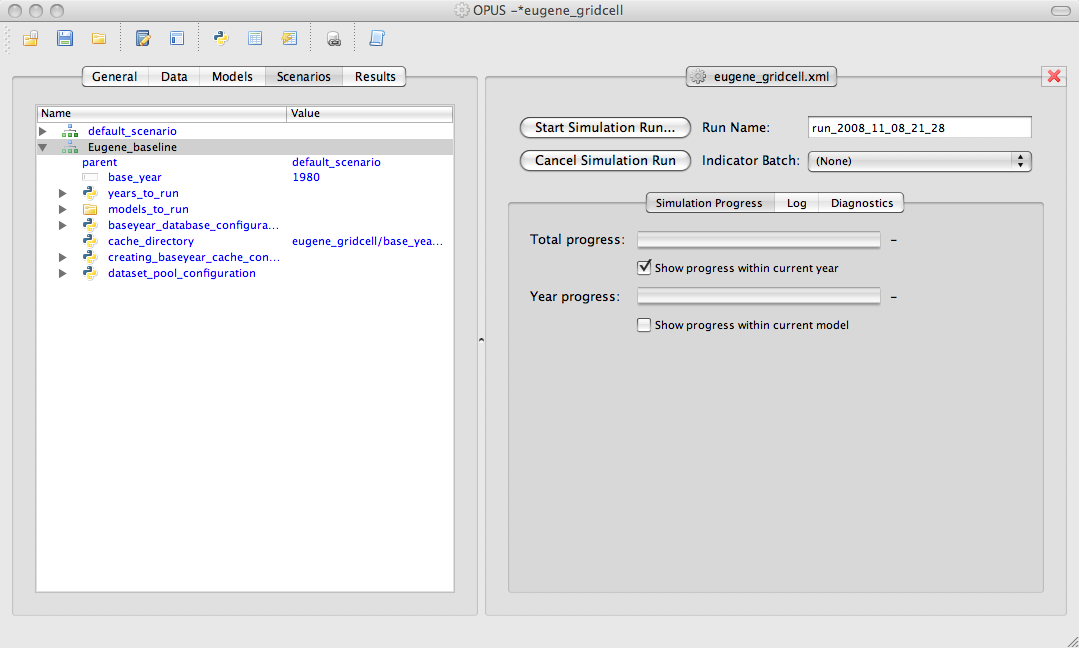
\includegraphics[scale=0.4]{part-gui/images/scenario-manager-start-run.png}
\end{center}
\caption{Starting a simulation on the Eugene baseline scenario}
\label{fig:scenario-manager-start-run}
\end{figure}

The frame on the right contains an option to start the simulation run and
another to cancel it.  Start the run with the
\verb#Start Simulation Run ...# button.  Note that the button's name
changes to \verb#Pause Simulation Run ...#.  The window will now update as
the simulation proceeds, with progress bars and labels being updated to
show the changing state of the system, such as which year the model is
simulating and which model is running.  If the simulation completes
successfully, the ``Total progress:'' bar will say ``Simulation ran
successfully'' after it, and the ``Year progress'' bar will say
``Finished'' (Figure \ref{fig:scenario-manager-completed-run}).

\begin{figure}[htp]
\begin{center}
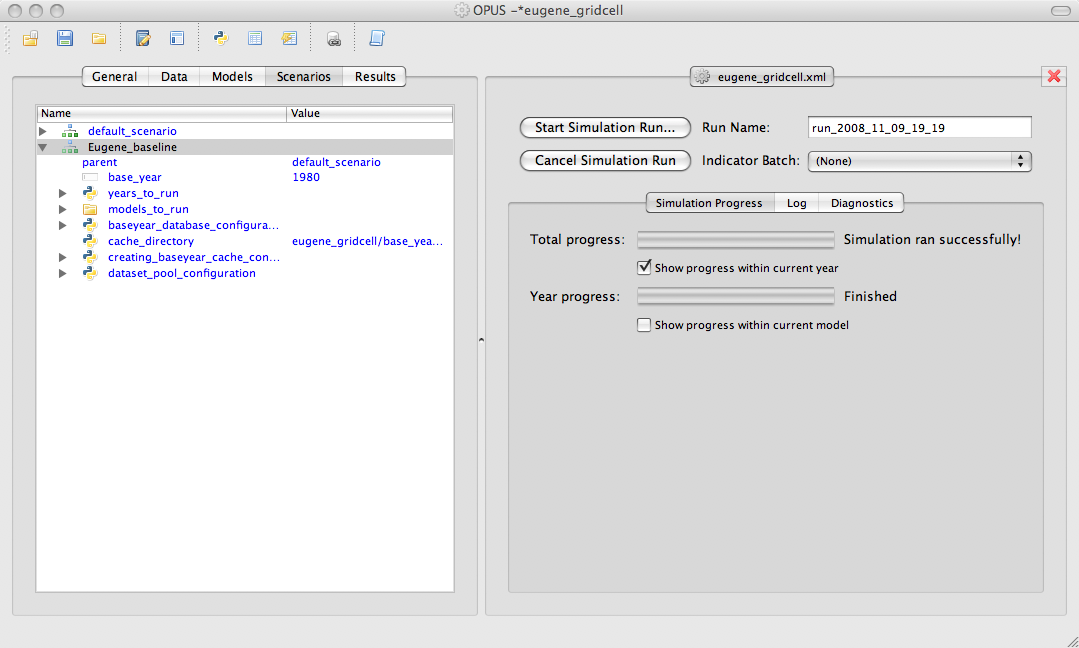
\includegraphics[scale=0.4]{part-gui/images/scenario-manager-completed-run.png}
\end{center}
\caption{A completed simulation run}
\label{fig:scenario-manager-completed-run}
\end{figure}

This simulation run then is entered into the simulation runs database,
which can be subsequently inspected via the ``Simulation\_runs'' node in
the Results Manager (Section \ref{sec:managing-simulation-runs}).
Indicator results from the simulation can also be generated using other
tools in the Results Manager (Section
\ref{sec:interrogating-results-with-indicators}).

That's it for the basics of running a simulation!  However, there are
various options for selecting, configuring and running a scenario, which
are described in the following subsections.

\subsection{Options for Controlling the Simulation Run}
\label{sec:controlling-simulation}

Here are the aspects of controlling the simulation run via controls in the
frame on the right.  The results of this simulation are entered into the
simulation runs database under the ``Run Name'' (upper right hand part of
the pane).  This is filled in with a default value consisting of ``run\_''
followed by the date and time; edit the field if you'd like to give the run
a custom name.  Immediately under that field is a combo box ``Indicator
Batch:''.  If you have defined and named a batch of indicators that can be
run, you can select one of these from the list, and the indicators will
automatically be run at the conclusion of the simulation.  See Section
\ref{sec:batch-indicator-configuration} for information on indicator
batches.

As mentioned above, once you start the simulation the
\verb#Start Simulation Run ...# button label changes to
\verb#Pause Simulation Run#\@.  If the pause button is pressed while the
model system is running, a request to pause the model is triggered, and
once the current model in the model system is finished, the system pauses
until you take further action by pressing either the
\verb#Resume Simulation Run...# or the \verb#Cancel Simulation Run# button.
The \verb#Cancel Simulation Run# button is also available while the
simulation is running.  (As with ``Pause,'' ``Cancel'' generally won't
happen immediately, but only after the current model in the model system is
finished.)

\subsection{Options for Monitoring the Simulation}
\label{sec:monitoring-simulation}

Moving down the frame, there is a button for selecting views in the bottom
of the screen.  The default is ``Simulation Progress,'' which shows
progress bars to allow you to track the simulation's activity.  The ``Log''
option shows a transcript with detailed simulation output.  Finally, the
``Diagnostics'' button supports generating on-the-fly diagnostic
indicators.  

\begin{figure}[htp]
\begin{center}
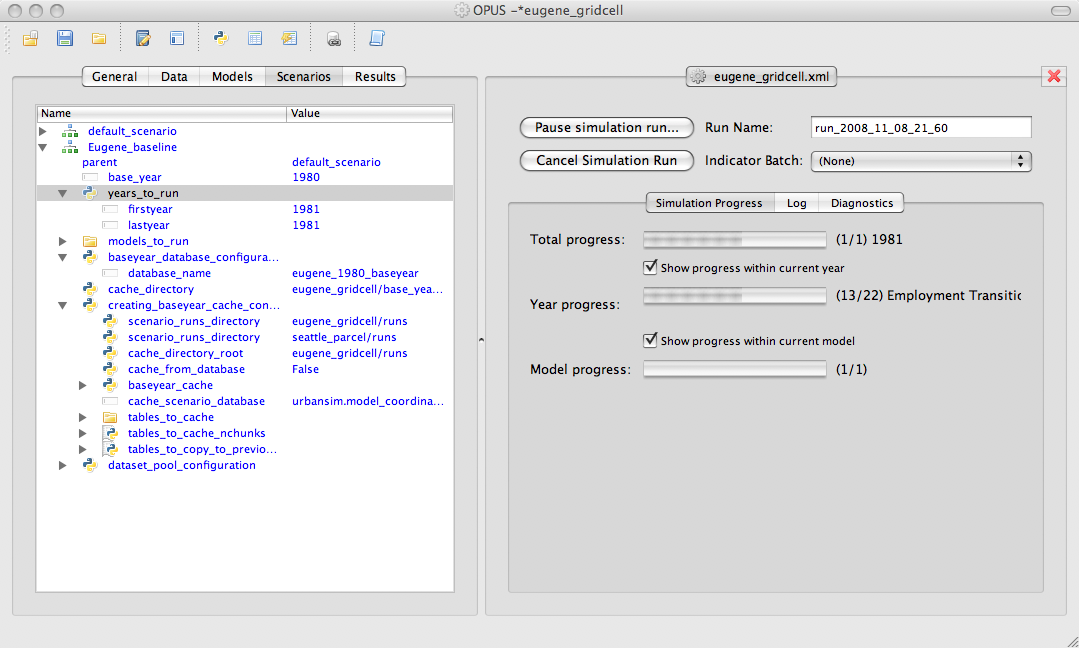
\includegraphics[scale=0.4]{part-gui/images/scenario-manager-progress-bars.png}
\end{center}
\caption{Running a simulation on Eugene baseline with all progress bars
  enabled}
\label{fig:scenario-manager-progress-bars}
\end{figure}

The default settings for ``Simulation Progress'' are to show the total
progress in running the simulation, and the progress within the current
year.  For example, if you are running for 10 simulated years, when the
first year is completed the progress bar for the current year will reach
100\% and the total progress will reach 10\%.  You can hide the progress
bar for the current year for a less cluttered display.  Finally, if ``Show
progress within current year'' is enabled, you have the additional option
(off by default) to show progress within each model, such as Employment
Transition, Household Transition, and so forth. The currently running year,
model, and chunk of model will be shown by the corresponding bars.  Figure
\ref{fig:scenario-manager-progress-bars} shows a running simulation with all
three progress bars enabled.

The ``Log'' option, as shown in Figure
\ref{fig:scenario-manager-log-pane.png}, shows the log output from running
the same scenario.  This can be monitored as the simulation runs, and also
consulted after it has completed.

\begin{figure}[htp]
\begin{center}
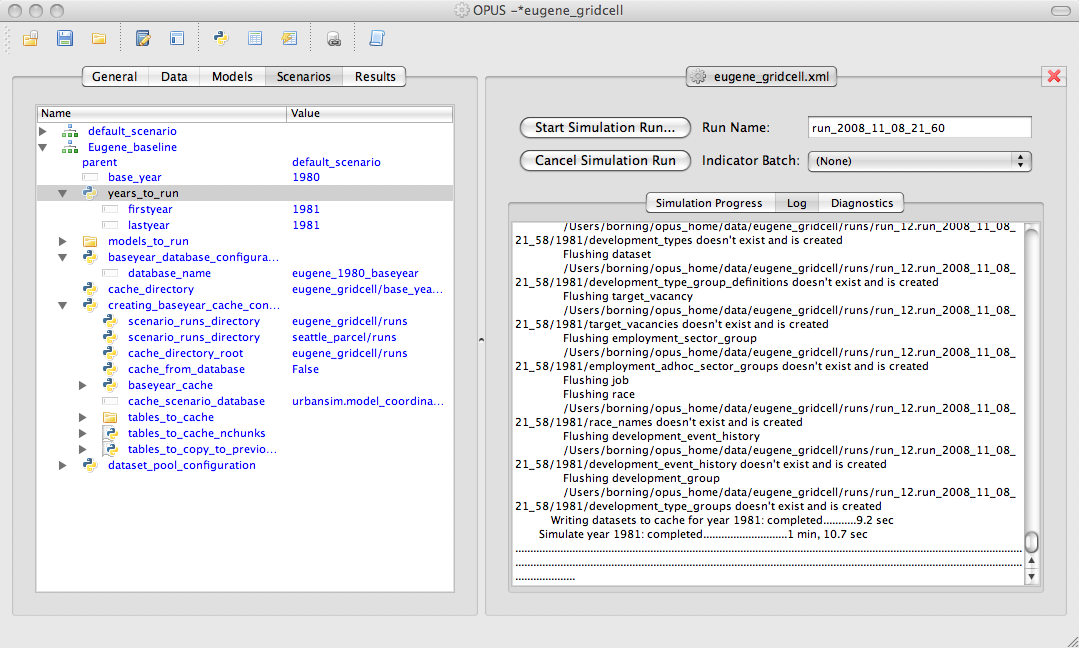
\includegraphics[scale=0.4]{part-gui/images/scenario-manager-log-pane.png}
\end{center}
\caption{Log information from running a scenario}
\label{fig:scenario-manager-log-pane.png}
\end{figure}

``Diagnostics,'' the last of these three options, supports generating
on-the-fly diagnostic indicators.  If this option is selected, a series of
combo boxes appears immediately below, allowing you to select a map or
chart indicator, the level of geography, a specific indicator, and the
year.  As the given simulated year completes, the corresponding indicator
visualization is shown underneath.  For example, Figure
\ref{fig:scenario-manager-diagnostic-map} shows a diagnostic map of population
for 1981 at the gridcell level for the Eugene baseline scenario.

\begin{figure}[htp]
\begin{center}
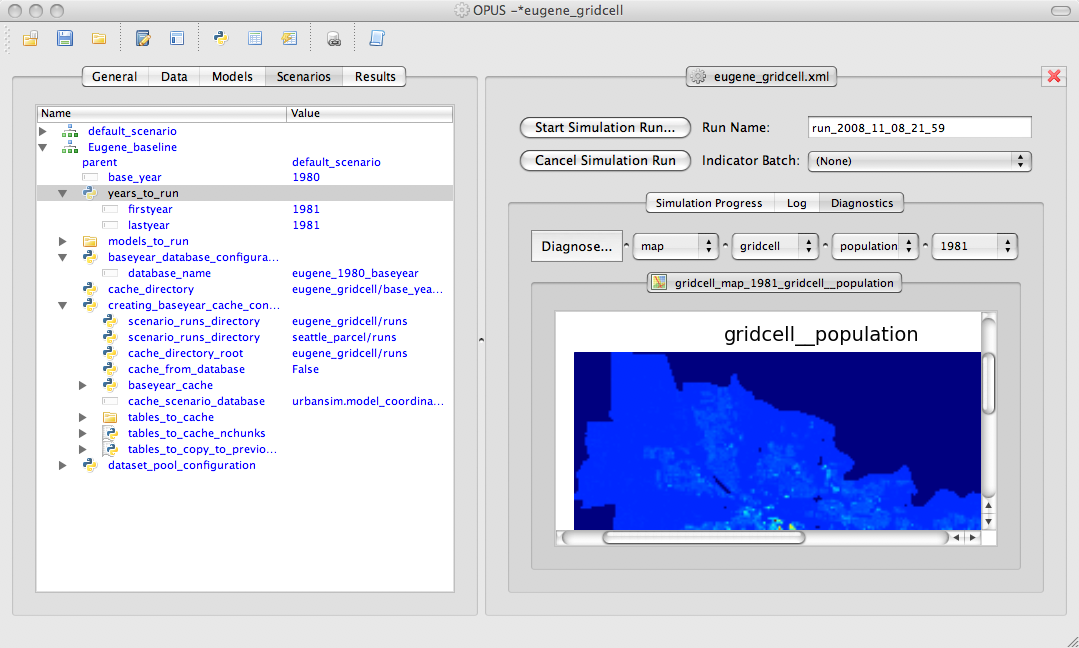
\includegraphics[scale=0.4]{part-gui/images/scenario-manager-diagnostic-map.png}
\end{center}
\caption{Using diagnostic indicators while running a scenario}
\label{fig:scenario-manager-diagnostic-map}
\end{figure}

\subsection{Selecting and Configuring a Scenario}
\label{sec:configuring-scenario}

To select a scenario to run or configure its options, use the XML tree view
on the left.

The default Eugene project contains only one scenario
(``Eugene\_baseline'').  However, in general projects can contain multiple
scenarios, all of which will be shown in the XML tree in the left-hand
pane.  Right-click on any one of them and select ``Run this Scenario'' to
run.

To change any of the options in the XML tree you need to be able to edit
it.  The initial version of the Eugene\_gridcell project in
\file{opus_home/project_configs/eugene_gridcell.xml} has basically no
content of its own --- everything is inherited from the default Eugene
gridcell configuration in the source code.  Inherited parts of the XML tree
are shown in blue.  These can't be edited directly --- they just show
inherited information.  Suppose that we want to change the last year of the
simulation run from 1981 to 1990.  To do this, first click on the triangle
next to \code{years_to_run} in the XML tree.  Right click on
\code{lastyear} and select ``Add to curent project.''  This copies the
inherited information into the local XML tree for the Eugene\_gridcell
configuration.  The \code{lastyear} entry turns black, and you can now edit
the year value to 1990.  After the options are set up as you would like,
you can then right click on the scenario and run it.  Figure
\ref{fig:scenario-manager-change-lastyear} shows the newly-edited scenario
being run for 10 simulated years.  (Notice that \code{lastyear} is now 1990
and shown in black.)

\begin{figure}[htp]
\begin{center}
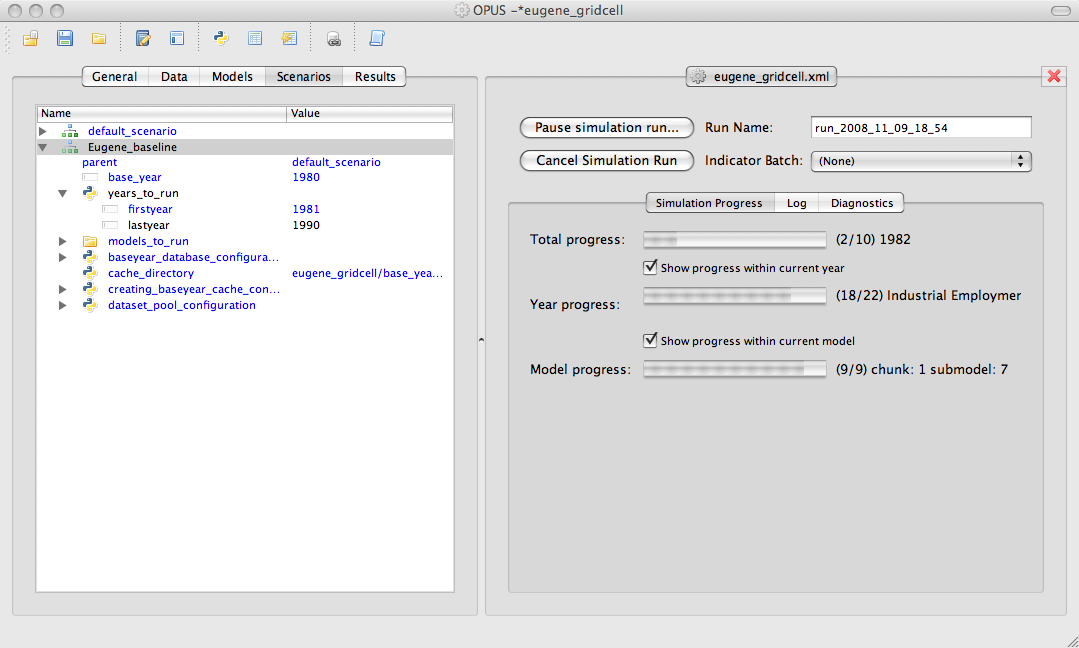
\includegraphics[scale=0.4]{part-gui/images/scenario-manager-change-lastyear.png}
\end{center}
\caption{Running a scenario after changing the last year to 1990}
\label{fig:scenario-manager-change-lastyear}
\end{figure}

The ending year of the scenario is the most likely thing that you'd want to
change.  Another possibility is to run only some of the component models.
To do this, right-click on ``Models to run,'' make it editable by
selecting ``Add to current project,'' and change the value of the ``Run''
field to ``Skip'' to skip that component model.

A few details about the ``Add to current project'' command: when you added
\code{lastyear} to the current project, the containing nodes in the tree
(\code{years_to_run} and \code{Eugene_baseline}) also turned black, since
they needed to be added to the current project as well to hold
\code{lastyear}.  It's also possible to click directly on
\code{years_to_run}, or even \code{Eugene_baseline}, and add the XML tree
under that to the current project.  However, we recommend adding just the
part you're editing to the current project, and not others.  (You can
always add other parts later.)  The reason is that once a part of the tree
is added to the current project, the inheritance relation of that part with
the parent disappears, and changes to the parent won't be reflected in the
child XML\@.  For example, if you add all of the \code{Eugene_baseline}
node to the current project, save your configuration, and then update the
source code, changes to some obscure advanced feature in the XML in the
parent in the source tree wouldn't show up in your configuration.
